\documentclass{beamer}
\usetheme[nat]{Frederiksberg}

\usepackage{algorithm}
\usepackage[noend]{algorithmic}
\usepackage{adjustbox}
\usepackage{multirow}
\usepackage{siunitx}
\usepackage{amsmath}

\begin{document}
\title{Master's thesis defense}
\author{Nikolaj Dybdahl Rathcke}
\date{June 27, 2018}

\frame{\titlepage}

% New page

\section{Motivation and Problem Definition}
\frame{\frametitle{Motivation and Problem Definition}
\begin{columns}[c]
  \column[b]{6cm}
  \begin{itemize}
    \item The \textit{distance oracle}.
    \item Performance measures
    \item The vertex-labeled variant.
  \end{itemize}
  \column{4cm}
  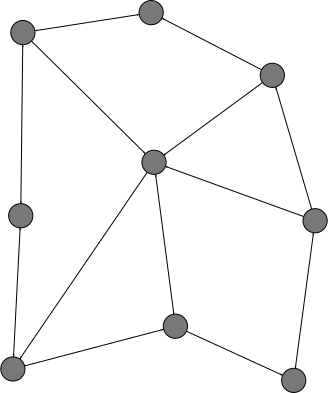
\includegraphics[width=\textwidth]{figs/intro.pdf}
\end{columns}

}

% New page

\section{Motivation and Problem Definition}
\frame{\frametitle{Motivation and Problem Definition}
\begin{columns}
  \column{6cm}
  \textbf{The distance oracle}. \\
  $ $ \\
  A compact data structure that can quickly answer shortest paths between two vertices $u$ and
  $v$.
  \column{4cm}
  \includegraphics[width=\textwidth]{figs/intro2.pdf}
\end{columns}

}

% New page

\section{Motivation and Problem Definition}
\frame{\frametitle{Motivation and Problem Definition}
\begin{columns}[c]
  \column{6cm}
  \textbf{Performance measures}. \\
  $ $ \\
  \textit{Space}. The size of the data structure. \\
  $ $ \\
  \textit{Query time}. The time it takes to answer shortest path queries. \\
  $ $ \\
  \textit{Preprocessing time}. The time it takes to build the data structure. \\
  $ $ \\
  \textit{Update time}. Time it takes to adjust the data structure
  to reflect changes to the graph.
  \column{4cm}
  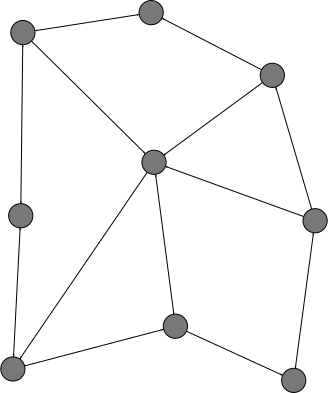
\includegraphics[width=\textwidth]{figs/intro.pdf}
\end{columns}

}

% New page

\section{Motivation and Problem Definition}
\frame{\frametitle{Motivation and Problem Definition}
\begin{columns}[c]
  \column{6cm}
  \textbf{The vertex-labeled variant}. \\
  $ $ \\
  Each vertex is associated with a label $\lambda$ from a set of labels $L=\{\lambda_1,
  \dots, \lambda_\ell\}$. \\
  Instead of answering shortest path between two vertices, we answer shortest path
  queries,  $Q(u,\lambda)$, from a vertex $u$ to the nearest $\lambda$-labeled vertex.
  \column{4cm}
  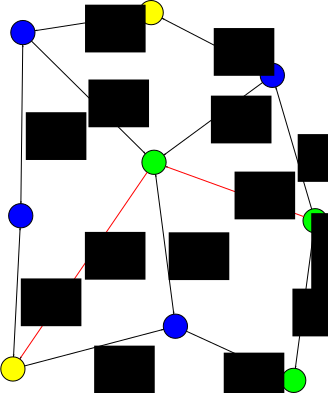
\includegraphics[width=\textwidth]{figs/intro3.pdf}
\end{columns}

}

% New page

\section{Motivation and Problem Definition}
\frame{\frametitle{Motivation and Problem Definition}
\begin{columns}[c]
  \column{6cm}
  \begin{itemize}
    \item The \textit{distance oracle}.
    \item Performance measures
    \item The vertex-labeled variant.
  \end{itemize}
  \noindent $ $\\
  \textbf{This thesis}: Distance oracles in directed planar vertex-labeled graphs.
  \column{4cm}
  \includegraphics[width=\textwidth]{figs/intro4.pdf}
\end{columns}

}

% New page

\section{Results}
\frame{\frametitle{Results}

  \begin{block}{Theorem 1}
    \small
    There is a distance oracle with space $O(n\ell^{2/3})$, query time $O(\ell^{1/3})$
    and preprocessing time \textcolor{red}{$\tilde{O}(n\ell^{2/3})$}.
  \end{block}
  \begin{block}{Theorem 2}
    \small
    There is a distance oracle that can handle edge-weight changes, edge insertions and
    deletion in amortized $\tilde{O}(n^{2/3})$ time. It can be constructed using
    $O(n\lg n)$ space in $O(n\lg n)$ time, and answers queries in
    $\tilde{O}(\min\{\text{size}(\lambda)\cdot n^{2/3}, n\})$ time.
  \end{block}
  \begin{block}{Theorem 3}
    \small
    Under the assumption that $G$ does not have $\omega(\sqrt{n})$ labels of polynomial
    size, there is a distance oracle with space $O(n^{3/2})$, query time
    $O(\text{polylog}(n))$ and preprocessing time \textcolor{red}{$\tilde{O}(n^{3/2})$}. Furthermore, it
    can handle labels changes in expected $O(1)$ time.
  \end{block}

}

% New page |||||| First oracle

\section{Warm-up: An oracle depending on $\ell$}
\frame{\frametitle{Warm-up: An oracle depending on $\ell$}

  \begin{block}{Theorem 1}
    \small
    There is a distance oracle with space $O(n\ell^{2/3})$, query time $O(\ell^{1/3})$
    and preprocessing time $\tilde{O}(n\ell^{2/3})$.
  \end{block}

\begin{columns}[c]
  \column{10cm}
  \begin{itemize}
    \item Built on top of an $r$-division.
    \item Store shortest paths to all labels from \textit{boundary vertices}.
    \item Store shortest paths from all \textit{interior vertices} to all labels in the
      same piece and to all boundary vertices of the piece.
  \end{itemize}
\end{columns}

}

% New page

\section{The $r$-division}
\frame{\frametitle{The $r$-division}

  Given some $r$, an $r$-division is a collection of connected subgraphs that satisfy:
  \begin{itemize}
      \item Any edge belongs to one region.
      \item There are $O(n/r)$ regions.
      \item For each region, there are $O(\sqrt{r})$ boundary vertices.
      \item For each region, there are $O(r)$ vertices.
  \end{itemize}
  \begin{center}
  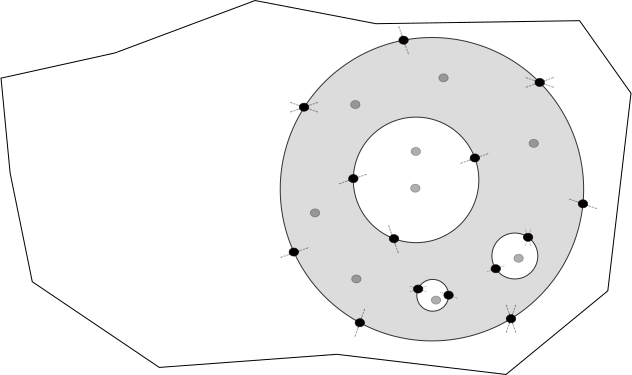
\includegraphics[scale=0.33]{figs/rdiv.pdf}
\end{center}

}

% New page

\section{The $r$-division}
\frame{\frametitle{The $r$-division}

  Given some $r$, an $r$-division is a collection of connected subgraphs that satisfy:
  \begin{itemize}
      \item Any edge belongs to one region.
      \item There are $O(n/r)$ regions.
      \item For each region, there are $O(\sqrt{r})$ boundary vertices.
      \item For each region, there are $O(r)$ vertices.
  \end{itemize}
  There is version due to Klein, Sommer and Mozes that further guarantees:
  \begin{itemize}
    \item Each region is a connected subgraph.
    \item Each region has $O(1)$ holes.
    \item Can be computed in $O(n)$ time.
  \end{itemize}

}

% New page

\section{The oracle}
\frame{\frametitle{The oracle}
  We store the following:
  \begin{itemize}
    \item Store shortest path from boundary vertices to all labels.
    \item Store shortest path from all interior vertices to all boundary vertices of the
      region as well as all labels inside the same
      region.
  \end{itemize}
  \begin{center}
  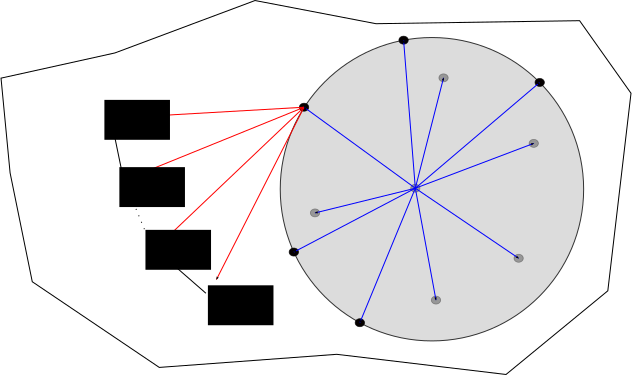
\includegraphics[scale=0.4]{figs/oracle1.pdf}
\end{center}

}

% New page

\section{The oracle}
\frame{\frametitle{The oracle}
  Given the query $Q(u,\lambda)$, find all distances $\delta(u,b)+\delta(b,\lambda)$ and
  the distance $\delta(u,\lambda)$ stored for $u$ inside the region. Return the minimum.
  \begin{center}
    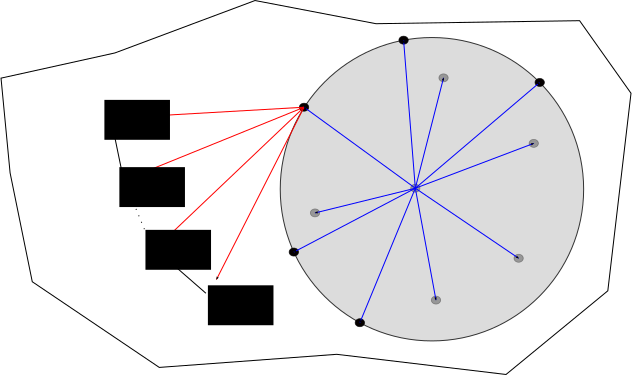
\includegraphics[scale=0.4]{figs/oracle1.pdf}
  \end{center}

}

% New page

\section{The oracle}
\frame{\frametitle{The oracle: Analysis}

  \textbf{Query}. Bounded by the number of boundary vertices, which is $O(\sqrt{r})$ \\
  $ $ \\
  \textbf{Space}. We have $O(n/r)$ regions, so $O(n/\sqrt{r})$ boundary vertices. For any
  interior vertex, we store up to $O(r)$ distances, yielding $O(n\ell/\sqrt{r}+nr)$
  space. \\
  $ $ \\
  \textbf{Preprocessing}. Compute SSSP from boundary vertices in $O(n)$ time. We then
  know distances between boundary vertices, so we can compute interior distances using
  Djikstra in $O(r\lg r)$ time. This gives us $O(n^2/\sqrt{r}+nr\lg r)$ preprocessing.

}

% New page

\section{The oracle}
\frame{\frametitle{The oracle: Analysis}

  \textbf{Query}: $O(\sqrt{r})$ \\
  \textbf{Space}: $O(n\ell/\sqrt{r}+nr)$ \\
  \textbf{Preprocessing}: $O(n^2/\sqrt{r}+nr\lg r)$ \\
  $ $ \\
  Pick $r=\ell^{2/3}$ to get Theorem 1:

  \begin{block}{Theorem 1}
    \small
    There is a distance oracle with space $O(n\ell^{2/3})$, query time $O(\ell^{1/3})$
    and preprocessing time \textcolor{red}{$\tilde{O}(n\ell^{2/3})$}.
  \end{block}

}

% New page |||||| Second oracle

\section{A dynamic vertex-labeled distance oracle}
\frame{\frametitle{A dynamic vertex-labeled distance oracle}

  \begin{block}{Theorem 2}
    \small
    There is a distance oracle that can handle edge-weight changes, edge insertions and
    deletion in amortized $O(n^{2/3}\lg^{5/3} n)$ time. It can be constructed using
    $O(n\lg n)$ space in $O(n\lg n)$ time, and answers queries in
    $\tilde{O}(\min\{\text{size}(\lambda)\cdot n^{2/3}, n\})$ time.
  \end{block}

\begin{columns}[c]
  \column{10cm}
  \begin{itemize}
    \item Built on an $r$-division.
    \item FR-Djikstra variant.
      \begin{itemize}
        \item Dense distance graph.
        \item Fast query using Djikstra and exploiting the Monge property in the DDG.
      \end{itemize}
    \item Henzinger's SSSP algorithm to avoid terrible worst-case times.
  \end{itemize}
\end{columns}

}

% New page

\section{The oracle}
\frame{\frametitle{The Dense Distance Graph}

  \begin{columns}
    \column{10cm}
    \begin{itemize}
      \item The complete graph on boundary vertices for each piece.
      \item Can be constructed in $O(n\lg r)$ time and $O(r\lg r)$ for a single region.
    \end{itemize}
  \end{columns}
  \noindent \\
  $ $ \\
  $ $ \\
  \centering
  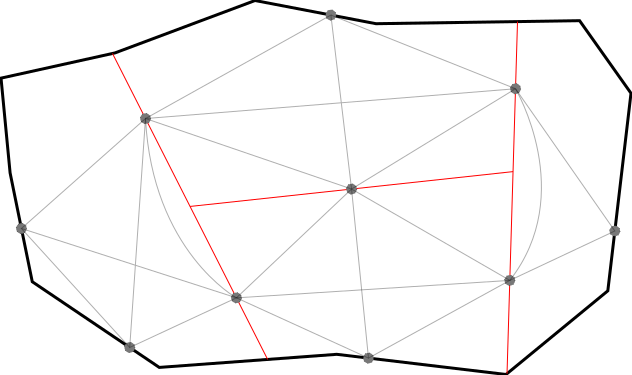
\includegraphics[scale=0.4]{figs/ddg.pdf}

}

% New page

\frame{\frametitle{The query}

  \small
  For query $Q(u,v)$, we do the following:
  \begin{itemize}
    \item Compute shortest path to boundary vertices from $u$ in $P_u$.
    \item Djikstra variant on boundary vertices in $O(n/\sqrt{r}\lg^2 n)$ time.
    \item Compute shortest path to $v$ in $P_v$ in $O(r)$ time.
    \item If same piece, check if this distance is smaller. For $Q(u,\lambda)$, total
      query time is $\tilde{O}(\text{size}(\lambda)\cdot r+n/\sqrt{r})$.
  \end{itemize}
  \centering
  \includegraphics[scale=0.4]{figs/ddgQ.pdf}

}

% New page

\frame{\frametitle{Updates}

  \small
  Only update $r$-division and DDG after an order of $\sqrt{r}$ of update operations have been performed.
  \begin{itemize}
    \item Edge weight changes, change weight and recompute DDG in $O(r\lg r)$ time.
    \item To delete and edge, we need to recompute the DDG of that piece in $O(r\lg r)$
      time.
    \item If an edge insertion is entirely within a piece, simply add it. Otherwise, we
      add another boundary vertex. Recompute DDG in $O(r\lg r)$ time.
  \end{itemize}
  \small
  We recompute an $r$-division and DDG after $\sqrt{r}$ operations, so an amortized
  analysis over all operations gives us $O(\frac{n+n\lg r}{\sqrt{r}}+r\lg r)=O(n\lg
  r/\sqrt{r}+r\lg r)$
    time per operation. \\

}

% New page

\frame{\frametitle{Theorem 2}

  \textbf{Space}: $O(n\lg n)$ \\
  \textbf{Preprocessing}: $O(n\lg n)$ \\
  \textbf{Query}: $\tilde{O}(\text{size}(\lambda)\cdot r + n/\sqrt{r})$ \\
  \textbf{Update}: $O(n\lg r/\sqrt{r}+r\lg r)$ \\
  $ $ \\
  Pick $r=n^{2/3}$ to get Theorem 2:

  \begin{block}{Theorem 2}
    \small
    There is a distance oracle that can handle edge-weight changes, edge insertions and
    deletion in amortized $\tilde{O}(n^{2/3})$ time. It can be constructed using
    $O(n\lg n)$ space in $O(n\lg n)$ time, and answers queries in
    $\tilde{O}(\min\{\text{size}(\lambda)\cdot n^{2/3}, n\})$ time.
  \end{block}

}

% New page |||||| Third oracle

\section{An oracle with better query times}
\frame{\frametitle{An oracle with better query times}

  \begin{block}{Theorem 3}
    \small
    Under the assumption that $G$ does not have $\omega(\sqrt{n})$ labels of polynomial
    size, there is a distance oracle with space $O(n^{3/2})$, query time
    $O(\text{polylog}(n))$ and preprocessing time $\tilde{O}(n^{3/2})$. Furthermore, it
    can handle label changes in expected $O(1)$ time.
  \end{block}

\begin{columns}[c]
  \column{10cm}
  \begin{itemize}
    \item Built on a recursive decomposition of $G$ using Jordan curves.
    \item Store all shortest paths to and from boundary vertices.
    \item Store \textit{additiviely weighted Voronoi diagrams} for all vertices $u$ and
      a constant number of holes $h$.
    \item Point to point distances in $O(\lg n)$ time using weighted Voronoi diagrams.
    \item Hash tables to keep track of what vertices have what labels.
  \end{itemize}
\end{columns}

}

% New page

\section{Additively weighted Voronoi diagrams}
\frame{\frametitle{Additively weighted Voronoi diagrams}

  \begin{columns}
    \column{6cm}
  \small
  When we separate a piece into two pieces $P$ and $Q$, a diagram is defined for a vertex
  $u\in P$ and hole $h$ of $Q$.
  \begin{itemize}
    \item \small Boundary vertices incident to $h$ are sites of the Voronoi diagram.
    \item \small A shortest path from $u$ to an interior vertex $v$ of $h$, will go through the site
      whose cell $v$ belongs to.
    \item \small We're after the representation, $VD^*$, which is a tree that requires $O(\sqrt{r})$ space.
  \end{itemize}
    \column{4cm}
  \includegraphics[scale=0.3]{figs/awvd1.pdf}
  $ $ \\
  $ $ \\
  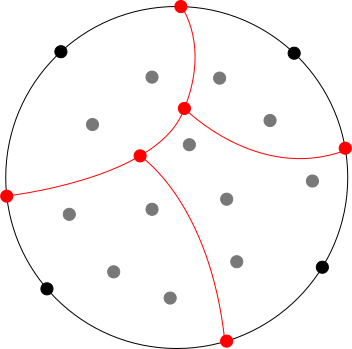
\includegraphics[scale=0.3]{figs/awvd2.pdf}
  \end{columns}

}

% New page

\frame{\frametitle{Point location}

  \begin{columns}
    \column{6.5cm}
  The stored information:
  \begin{itemize}
    \item \small We have stored shortest path trees from all boundary vertices.
    \item \small For vertices of $VD^*$, we store the distance from the three adjacent
      sites.
    \item \small The centroid decomposition of $VD^*$.
  \end{itemize}
  For the query $Q(u,v)$:
  \begin{itemize}
    \item \small Travel $VD^*$, compare distance from $u$ to $v$ for the three adjacent sites to
      $v^*$.
    \item \small Say site $s$ is closest, we can travel two edges. Locate $v$ relative to the
      shortest path from $s$ to $v^*$ and travel down the corresponding edge of $VD^*$.
  \end{itemize}
    \column{3.5cm}
  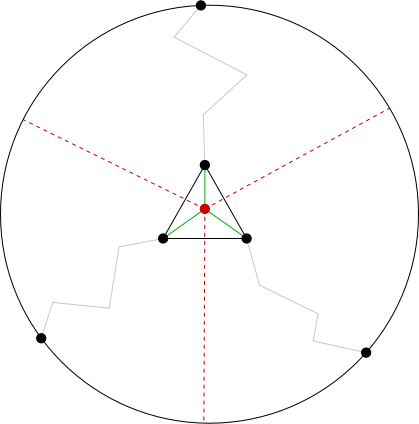
\includegraphics[width=\textwidth]{figs/vd2.pdf}
  $ $ \\
  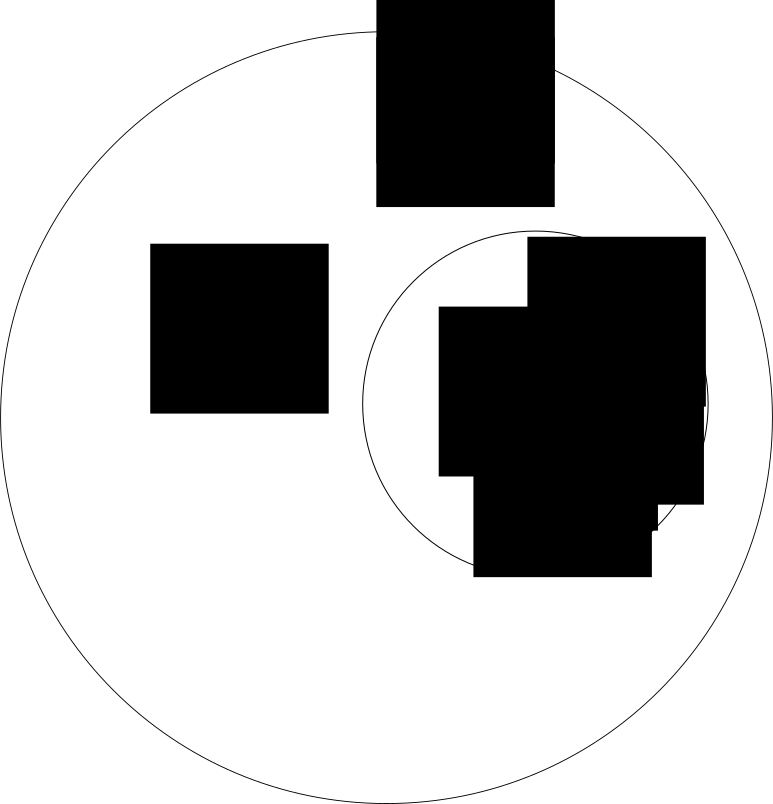
\includegraphics[width=\textwidth]{figs/vd1.pdf}
  \end{columns}

}

% New page

\section{The oracle}
\frame{\frametitle{The oracle}

  The additively weighted
  Voronoi diagrams allow point to point location in $O(\lg n)$ time. For labels that
  are polynomial in size, we store shortest paths directly.
  \begin{itemize}
    \item Check size of label. If it is polynomial, lookup distance in $O(1)$ time.
    \item If not, we make $\text{size}(\lambda)$ point to point queries.
    \item Travel decomposition tree. If either $u$ or $v$ is part of a separator, we can
      lookup the distance. If they belong to the same piece, we descend into that piece.
      If they belong to different pieces, we make point locations point locations in the
      additively weighted Voronoi diagrams stored for $u$.
  \end{itemize}

}

% New page

\frame{\frametitle{Handling label changes}

  We can extend the oracle to handle label changes in expected amortized $O(1)$ time.

  \begin{itemize}
    \item Add a hash table that keeps track of labels on vertices.
    \item A dynamic version of the hash table that return all vertices given a label.
      $\lambda$.
  \end{itemize}

}

% New page

\frame{\frametitle{The oracle: Analysis}

  \small
  \textbf{Space}: We store shortest path to and from boundary vertices requiring
  $O(n^{3/2})$ space. Each of the $O(1)$ additiviely weighted Voronoi diagram stored for
  a vertex $u$ requires worst case $O(\sqrt{n})$ space, totalling $O(n^{3/2})$. For
  labels of polynomial size, we use $O(n^{3/2})$ space under the simplifying assumption.
  \\
  $ $ \\
  \textbf{Query}: For labels of polynomial size, this takes $O(1)$ time. Otherwise, we
  descend into the decomposition tree of depth $O(\lg n)$ followed by $O(1)$ queries
  to the point location structure taking $O(\lg n)$ time. Since we do this at most $O(\text{polylog}(n))$
  times, this dominates the query time.

}

\frame{\frametitle{The oracle: Analysis}

  \small
  \textbf{Preprocessing}: The shortest path trees for boundary vertices can be computed
  in $O(n^{3/2})$ time. For labels of polynomial size (of which there at most
  $O(\sqrt{n})$ of), we can compute the shortest paths in $\tilde{O}(n^{3/2})$ time.
  All distances for the additively weighted Voronoi diagrams are already computed, so we
  can construct these in $O(|P|)$ time and extend them in $O(\sqrt{|P|})$ time to support
  point location. There are $O(n)$ of these, for a total of $O(n|P|)$. Total time spent is
  $O(n^{2})$. \\
  $ $ \\
  \textbf{Update}: Under the assumption that label sizes do not become polynomial, we
  have the load factor $\alpha$ is less than one, which means we can expect amortized
  $O(1)$ time for updates. Space is linear.

}

% New page

\frame{\frametitle{Putting it together}

  \small
  \textbf{Space}: $O(n^{3/2})$ \\
  \textbf{Query}: $O(\text{polylog}(n))$ \\
  \textbf{Preprocessing}: $\tilde{O}(n^{3/2})$\\
  \textbf{Update}: $O(1)$. \\
  $ $ \\
  This gives us our main Theorem:

  \begin{block}{Theorem 3}
    \small
    Under the assumption that $G$ does not have $\omega(\sqrt{n})$ labels of polynomial
    size, there is a distance oracle with space $O(n^{3/2})$, query time
    $O(\text{polylog}(n))$ and preprocessing time \textcolor{red}{$\tilde{O}(n^{3/2})$}. Furthermore, it
    can handle labels changes in expected $O(1)$ time.
  \end{block}

}

% New page

\section{Conclusion and future work}
\frame{\frametitle{Conclusion and future work}

  \begin{itemize}
    \item Exact distance oracles for Vertex-labeled planar graphs is unexplored.
    \item The goal was to match trade-offs given for regular distance oracles.
    \item A result based on $\ell$ providing us with trade-off for space-query.
    \item A result based on FR-Djikstra to show we can handle edge modifications For this
      type of graph
    \item A result which almost matches the best results for non vertex-labeled graphs,
      and works for most graphs.
    \item Removing the assumption.
    \item Extend to other classes of graphs.
  \end{itemize}

}

% New page

\frame{\frametitle{The end}

  Thanks to Christian Wulff-Nilsen for supervising the project. \\
  $ $ \\
  \centering
  \Huge Questions?

}



\end{document}
